\documentclass{beamer}
%
% Choose how your presentation looks.
%
% For more themes, color themes and font themes, see:
% http://deic.uab.es/~iblanes/beamer_gallery/index_by_theme.html
%
\mode<presentation>
{
  \usetheme{default}      % or try Darmstadt, Madrid, Warsaw, ...
  \usecolortheme{default} % or try albatross, beaver, crane, ...
  \usefonttheme{default}  % or try serif, structurebold, ...
  \setbeamertemplate{navigation symbols}{}
  \setbeamertemplate{caption}[numbered]
} 

\usepackage[english]{babel}
\usepackage[utf8x]{inputenc}
\usepackage{multirow}
\usepackage{booktabs}
\usepackage{bigstrut}
\usepackage{hyperref}


\begin{document}




\begin{frame}{Experiments}

\begin{itemize}
    \item \textbf{Superposition}  Combine the purchasing history of the $K$ neighbors and the prespecified user $u$. The Hawkes process has $D^{super}$ dimensionals.
    \item \textbf{Learning} Learn the parameters $\mu$ and $A$ from the history.
    \item \textbf{Prediction} Leverage the history and the parameters to compute intensity function. Use Ogata's modidified thinning algorithm to simulate.

    
\end{itemize}
    
    
\end{frame}











\begin{frame}{Experiments}


\begin{figure}
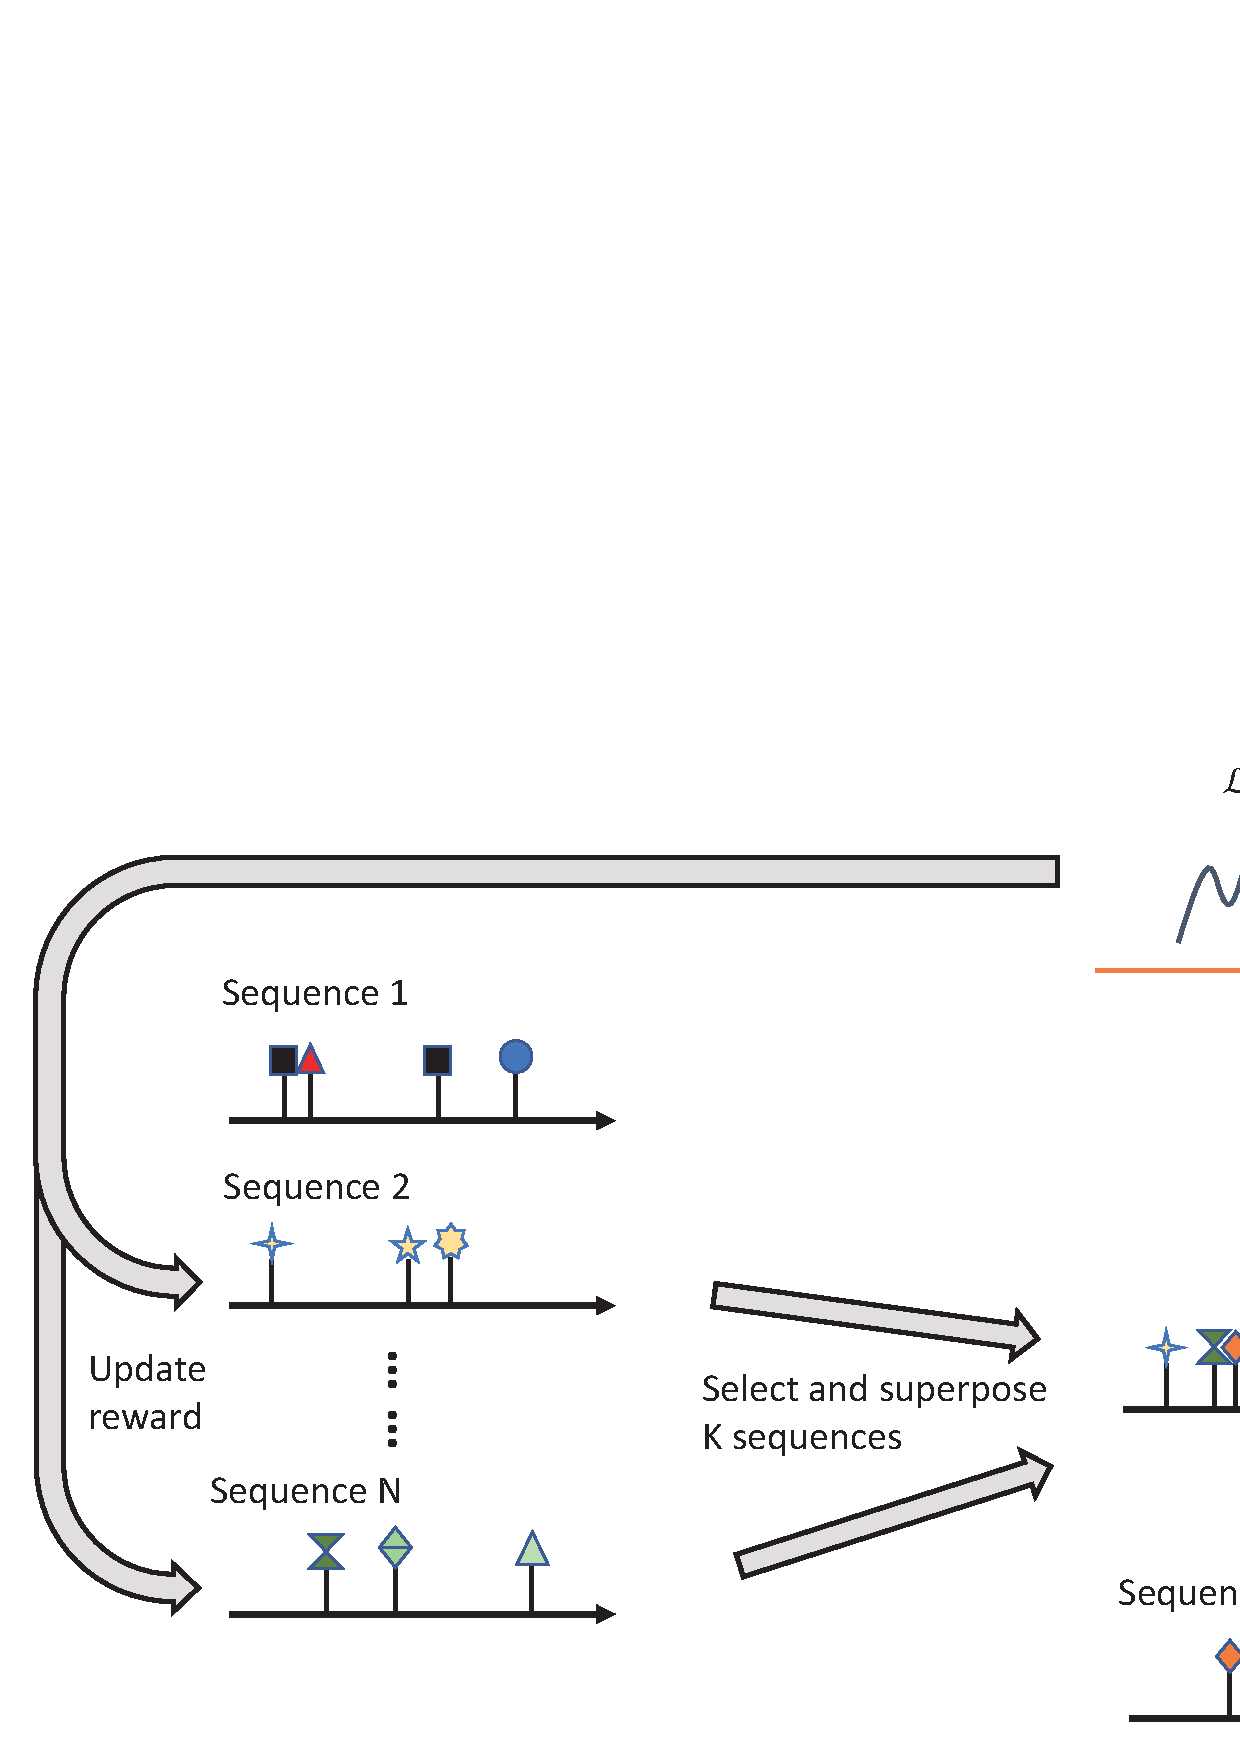
\includegraphics[height=2.7cm]{figure1.png}
\caption{The superposed history}
\end{figure}

\begin{figure}
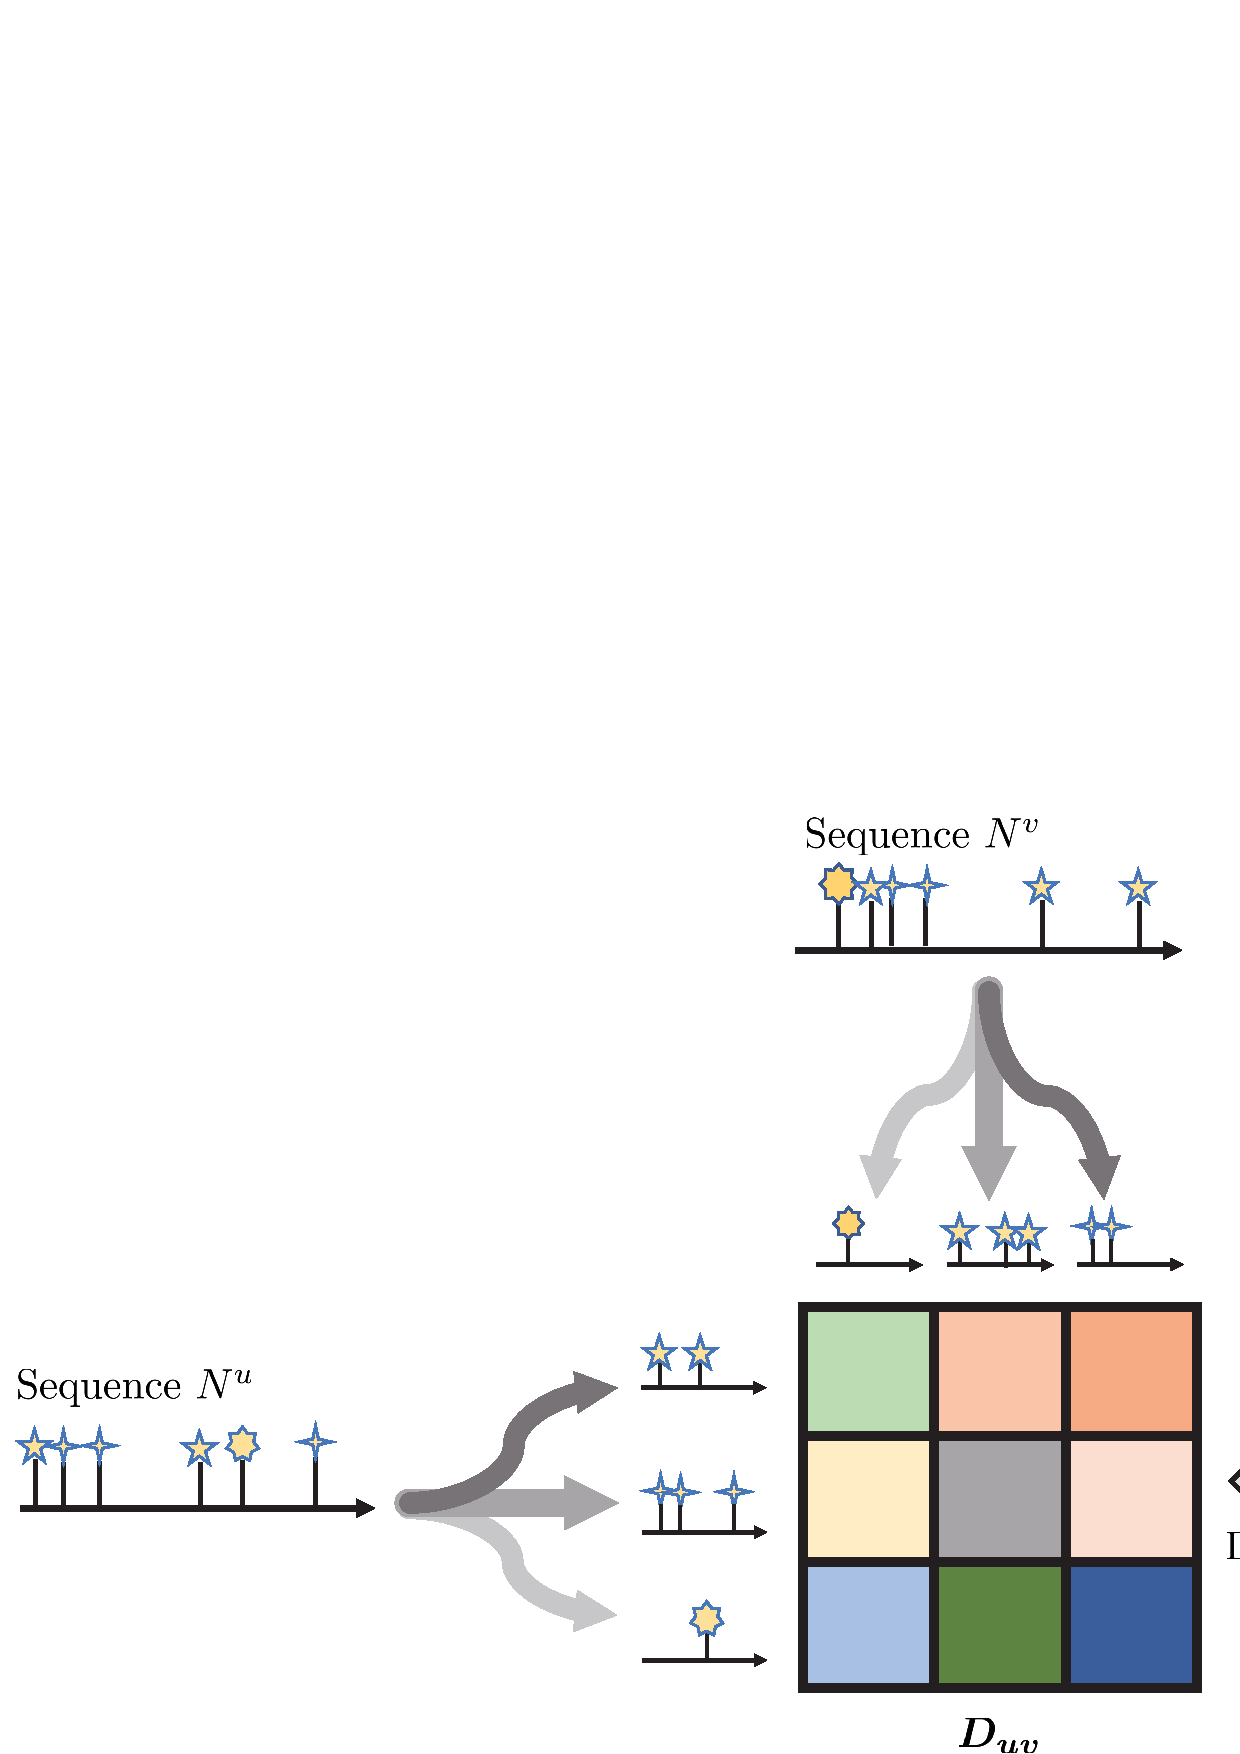
\includegraphics[height=1.1cm]{figure2.png}
\caption{Results of simulation}
\end{figure}

\begin{figure}
\includegraphics[height=0.9cm]{figure3.png}
\caption{Results of simulation}
\end{figure}


\end{frame}



\end{document}
